\documentclass[a4paper,12pt]{report}

\usepackage{alltt, fancyvrb, url}
\usepackage{graphicx}
\usepackage[utf8]{inputenc}
\usepackage{float}
\usepackage{hyperref}
\usepackage{adjustbox}
\usepackage{siunitx}
\usepackage{tabularx}
\sisetup{group-separator={\text{\space}}}

\usepackage[italian]{babel}

\usepackage[italian]{cleveref}

\title{Relazione di progetto \\``Programmazione di reti''\\Traccia 1 - Progetto DRONI}

\author{Nicolò Guerra \and
Emma Leonardi \and
Filippo Casadei 
}

\begin{document}

\maketitle

\tableofcontents

\chapter{Analisi dei requisiti}

Si ipotizzi di dover gestire una rete di consegne di piccoli pacchi a domicilio tramite l’utilizzo di droni. La rete è
composta da:

\begin{itemize}
    \item un client da cui l’operatore assegna a ciascun drone l’indirizzo di consegna del pacco
    \item tre droni
    \item un gateway che provvede ad effettuare il relay dei messaggi verso i droni e a fare da concentratore per raccogliere i messaggi provenienti dai droni ed inviarli al client
\end{itemize}

Il client deve poter inviare l’indirizzo di consegna del pacco ad un drone, solo dopo che lo stesso drone si sia
presentato al gateway come «disponibile». La connessione tra droni e gateway è di tipo UDP mentre la
connessione tra client e gateway è di tipo TCP.
Ogni drone ha un suo indirizzo IPv4, e cosi le due interfacce del gateway e il client.
Sulla console del client si deve poter inserire l’indirizzo di consegna del pacco e l’identificativo (o anche l’ip
address) del drone che dovrà effettuare la consegna. Tali informazioni devono essere inviate al gateway che
provvederà ad inviare l’informazione sulla destinazione del pacco al drone incaricato. Tali informazioni devono
essere visibili sulla console del gateway.
Infine sulla console del Drone dovrà essere visibile l’indirizzo di destinazione del pacchetto. Il drone dovrà quindi
inviare al gateway un messaggio di avvenuta consegna del pacchetto (ipotizzare un tempo randomico in un
intervallo a scelta) e rendersi nuovamente disponibile.
Sulla console del gateway devono comparire tutti i messaggi in transito con sorgente e destinatario.
I 3 droni hanno un indirizzamento appartenente ad una rete di Classe C del tipo 192.168.1.0/24
Il Gateway ha due interfacce di rete: quella verso i droni il cui IP Address appartiene alla stessa network dei dispositivi mentre l’interfaccia verso il client ha indirizzo
ip appartenente alla classe 10.10.10.0/24, classe a cui appartiene anche l’IP address del gateway.
Si realizzi un emulatore Python che sfruttando il concetto dei socket visti in laboratorio consenta di simulare, utilizzando l’interfaccia di loopback del proprio PC, il
comportamento di questo sistema.
Si devono simulare le conessioni UDP dei device verso il Gateway e la connessione TCP del Gateway verso il Client. Inoltre indicare la dimensione dei buffer utilizzati
su ciascun canale trasmissivo, il tempo impiegato per trasmettere il pacchetto UDP ed il tempo impiegato per trasmettere il pacchetto TCP.

\chapter{Trasporto}

La dimensione dei vari buffer utilizzati nel progetto è di 1024 byte. 
\section{Comunicazione tra gateway e client}
La comunicazione tra gateway e client è di tipo TCP, è quindi semplice da realizzare poichè non richiede alcun tipo di controllo di trasmissione.
\section{Comunicazione tra droni e gateway}
La comunicazione tra droni e gateway è di tipo UDP, che essendo di tipo best effort non garantisce la consegna dei pacchetti, si deve quindi implementare un controllo 
di trasmissione. Per questo si è utilizzato una sequenza di messaggi di controllo, in particolare ogni volta che il gateway o il drone ricevono un messaggio, inviano a 
loro volta un messaggio di controllo "OK" in risposta. Se il drone o il gateway non ricevono il messaggio di controllo procedono con un tentativo di ritrasmissione in una
finestra di tempo di 4 secondi, per un massimo di 5 tentativi, prima di considerare l'altro host non raggiungibile.

\begin{figure}[p]
    \begin{adjustbox}{addcode={\begin{minipage}{\width}}{\caption{%
      Schema di Trasmissione.
      }\end{minipage}},rotate=270,center}
      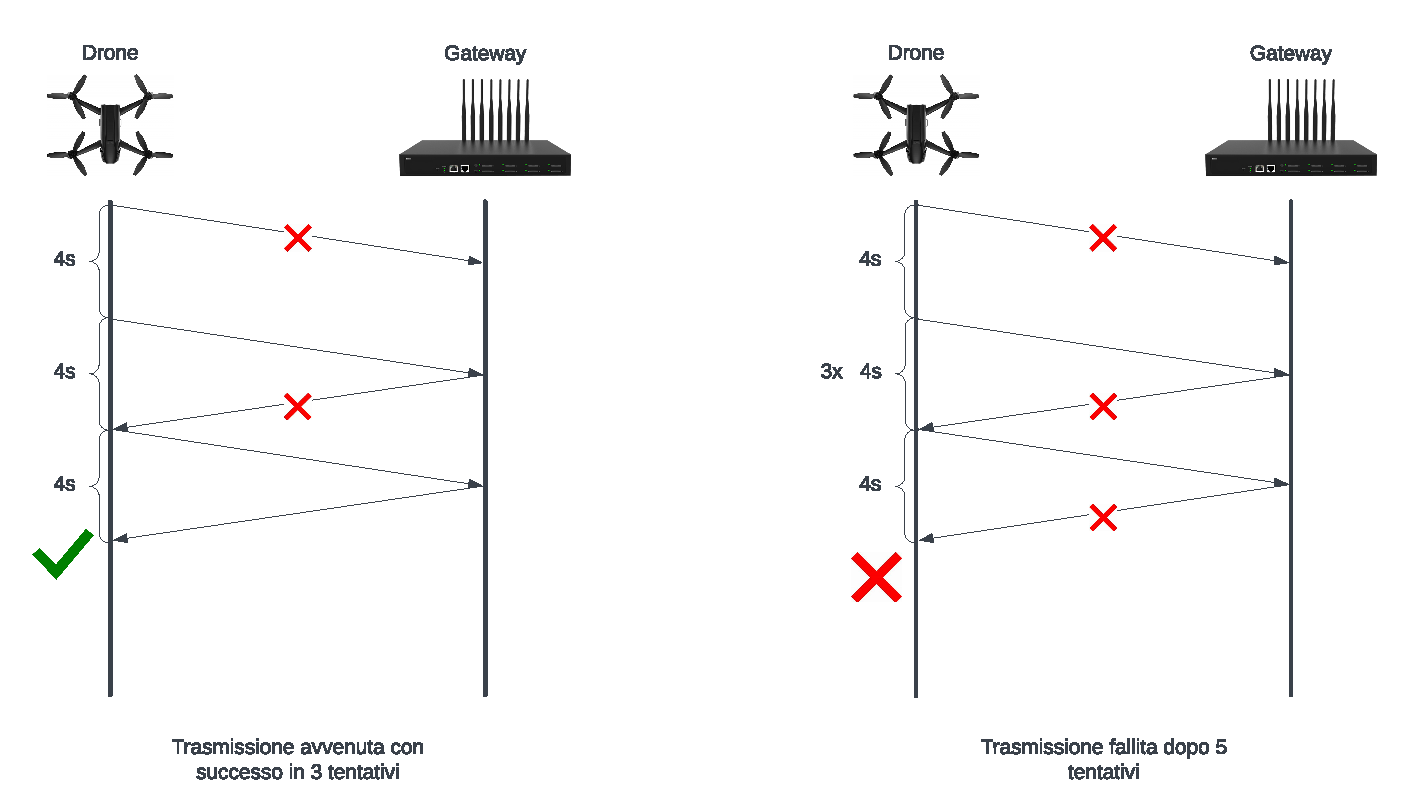
\includegraphics[height=0.93\textwidth]{img/trasmissions.pdf}
      \label{img:er}
    \end{adjustbox}
 \end{figure}

\chapter{Protocolli}
Tutti i comandi sono trasmessi come una lista di campi separati da ":". 
Per le comunicazioni verso il gateway il primo campo è l'indirizzo IP del mittente (solo a scopo di simulazione, in un contesto reale verrebbe utilizzata la sessione TCP 
nel caso del client, o i dati del pacchetto UDP nel caso del drone), il secondo campo è il comando da eseguire e infine i campi successivi sono i parametri necessari 
all'esecuzione del comando.
Per le comunicazioni in uscita dal gateway non viene trasmesso l'IP in quanto sia i droni che il client lo devono già conoscere a priori per potersi connettere.
\section{Comunicazione tra gateway e client}
\begin{itemize}
    \item \textbf{cregister}: inviato da client a gateway all'inizio della connessione, permette di registrare il client presso il gateway.
    \item \textbf{drones}: inviato da client a gateway, permette di ottenere la lista dei droni in forma di dictionary (ip-porta).
    \item \textbf{deliver}: inviato da client a gateway, permette di richiedere una consegna di un drone a un indirizzo.
    \item \textbf{ping}: inviato da client a gateway, per calcolare il tempo di risposta in millisecondi.
\end{itemize}
\section{Comunicazione tra droni e gateway}
\begin{itemize}
    \item \textbf{register}: inviato da drone a gateway, registra un drone come libero presso il gateway.
    \item \textbf{unregister}: inviato da drone a gateway, permette a un drone di disconnettersi dal gateway.
    \item \textbf{deliver}: inviato da drone a gateway, permette di richiedere una consegna di un drone a un indirizzo.
    \item \textbf{delivered}: inviato da drone a gateway, indica che un drone ha consegnato un pacco.
\end{itemize}

\chapter{Implementazione}
\section{Schema thread}
\begin{figure}[H]
	\centering{}
	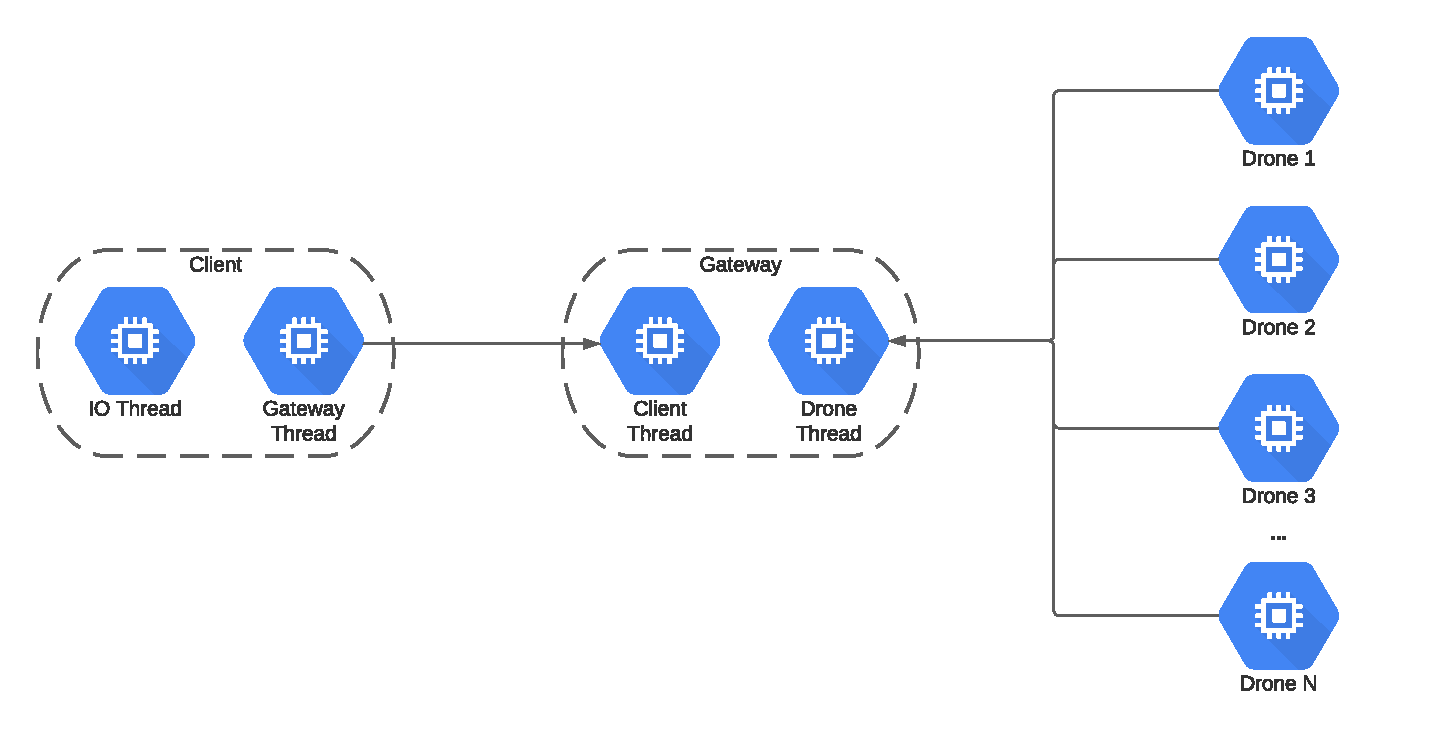
\includegraphics[width=\textwidth]{img/threads.pdf}
	\caption{Schema threads del sistema.}
	\label{img:scheletro}
\end{figure}

\paragraph*{Droni:} Ogni drone è gestito da un thread che si occupa di ricevere e inviare i messaggi di comunicazione verso il gateway e di effettuare le consegne.
\paragraph*{Gateway:} Il gateway è gestito da due threads che si occupano rispettivamente di comunicare con i droni e con il client. Per gestire le consegne il thread che comunica
con il client inserisce la consegna da effettuare in una lista che viene svuotata a intervalli regolari dal thread che comunica con i droni. In questo modo
si garantisce con l'uso di una lock la mutua esclusione e solo un thread comunica su una determinata socket.
\paragraph*{Client:} Il client è gestito da due thread. Il primo thread ascolta sul socket collegato al gateway e si occupa di mostrare i messaggi in arrivo. 
Il secondo thread è quello che gestisce l'input/output con l'utente. In questo modo, l'attesa per l'input esterno non blocca l'arrivo dei messaggi dal gateway 
come sarebbe successo se il tutto fosse stato gestito da un unico thread.

\appendix
\chapter{Guida utente}

Per avviare il sistema è necessario eseguire il gateway, che all'avvio si metterà in ascolto sulle porte 25000 per i droni e 26000 per il client.
A questo punto è possibile avviare il client e i droni, che si connetteranno al gateway. I droni cercheranno di connettersi finchè non troveranno un gateway
disponibile. Il client invece cercherà di connettersi e qualora non trovasse nessun gateway terminerà.

È possibile inviare comandi dalla console del client e questi verranno eseguiti dal gateway dopo essere stati visualizzati anche su quest'ultimo. In qualunque momento è possibile
interrompere il sistema digitando "exit", o tornare al menu iniziale digitando "-1".
Qualora si dovesse chiudere il client il gateway rimarrà aperto attendendo una nuova connessione dal client.
È possibile mandare una richiesta al gateway di visualizzare quali droni sono connessi con il comando "drones" quando si è nel menù di input indirizzo. La scelta del drone da 
utilizzare per la consegna è da fare specificando l'indirizzo IP. Il client inoltre ha il comando "ping" che invia al gateway una richiesta per vedere sulla console il tempo di risposta in millisecondi.
È possibile terminare uno qualunque dei componenti con l'interrupt da tastiera CTRL+C.

\chapter{Divisione del progetto}
La realizzazione dei vari componenti è stata divisa tra i membri del gruppo, ognuno dei quali ha effettuato i test necessari per la propria parte e infine un test generale per
verificare il funzionamento dell'interazione tra gateway, client e droni.
Seguono i membri con il lavoro a loro assegnato
\begin{itemize}
    \item Filippo Casadei, sviluppo dei droni\\ email: \url{filippo.casadei9@studio.unibo.it}\\ Matricola: 0000971563
    \item Emma Leonardi, sviluppo del client\\ email: \url{emma.leonardi2@studio.unibo.it}\\ Matricola: 0000971438
    \item Nicolò Guerra, sviluppo del gateway\\ email: \url{nicolo.guerra@studio.unibo.it} \\ Matricola: 0000971562
\end{itemize}

\end{document}